\documentclass[../TDE6_rsf.tex]{subfiles}%

\begin{document}
\section[s]"1"{Circuit RL série en RSF}
\enonce{%
	\noindent
	\begin{minipage}[t]{.6\linewidth}
		On considère le circuit ci-contre en régime sinusoïdal forcé, où la source de
		tension impose $e(t) = E\cos(\wt)$ avec $E > 0$.
	\end{minipage}
	\hfill
	\begin{minipage}{0.35\linewidth}
		\begin{center}
			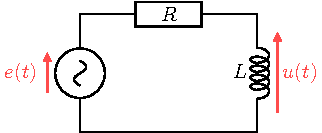
\includegraphics[width=\linewidth]{rl_rsf}
		\end{center}
	\end{minipage}
}

\QR{%
	Déterminer l'amplitude de $u$ à «~très haute~» ($\w\ra\infty$)
	et «~très basse~» ($\w\ra0$) fréquence.
}{%
	Pour les comportements limites, on utilise la modélisation d'une
	bobine à haute et basse fréquence~: étant donné que $\Zu_L = \jj L
		\w$, pour $\w\ra0$ on a $\Zu_L = 0$, et pour
	$\w\ra\infty$ on a $\Zu_L \ra \infty$. On a donc
	respectivement un fil et un interrupteur ouvert. En effet, l'impédance
	étant homogène à une résistance, une impédance nulle est semblable à une
	résistance nulle (un fil), et une impédance infinie est semblable à une
	résistance infinie (un interrupteur ouvert).
	\smallbreak
	\noindent
	\begin{isd}
		\tcbsubtitle{\fatbox{\textbf{$\w\to 0$}}}
		\begin{center}
			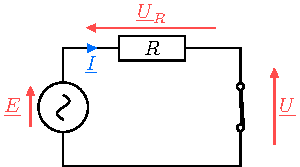
\includegraphics[scale=1]{rl_rsf-bf}
		\end{center}
		Or, la tension d'un fil est nul, donc
		\[\boxed{u \xrightarrow[\w\ra0]{} 0}\]
		\tcblower
		\tcbsubtitle{\fatbox{\textbf{$\w\to \infty$}}}
		\begin{center}
			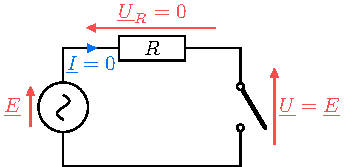
\includegraphics[scale=1]{rl_rsf-hf}
		\end{center}
		Le courant ne peut traverser un interrupteur, donc en faisant la loi des
		mailles dans le circuit équivalent, on a $u_R = Ri = 0$, et forcément
		\[\boxed{u \xrightarrow[\w\ra\infty]{} E}\]
	\end{isd}
}

\QR{%
	Exprimer l'amplitude complexe $\Uu$ de $u(t)$ en fonction de $E$,
	$R$, $L$ et $\w$.
}{%
	\smallbreak
	\noindent
	\begin{isd}
		\begin{center}
			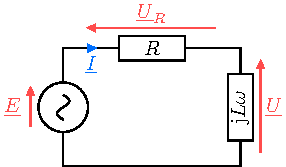
\includegraphics[scale=1]{rl_rsf-cplx}
		\end{center}
		\tcblower
		Pour cela, on utilise la relation du pont diviseur de tension~:
		\begin{gather*}
			\Uu
			= \frac{\Zu_L}{\Zu_L + \Zu_R}E
			\Lra
			\boxed{\Uu
				= \frac{\jj L\w}{R + \jj L \w}E}
		\end{gather*}
	\end{isd}
}

\QR{%
	Les tensions $e$ et $u$ peuvent-elles être en phase~? En opposition de
	phase~? En quadrature de phase~? Préciser le cas échéant pour quelle(s)
	pulsation(s).
}{%
	La phase de $e(t)$ est nulle par construction. On calcule donc la
	phase de $u$ en prenant l'argument de son amplitude complexe~:
	\begin{gather*}
		\arg*{\Uu}
		= \arg*{\jj L\w E} - \arg{\underbracket[1pt]{R}_{\mathclap{\Re > 0}} + \jj L \w}
		= \frac{\pi}{2} - \arctan \left( \frac{L\w}{R} \right)
	\end{gather*}
	où on peut prendre l'arctangente parce que la partie réelle est
	positive. Ainsi~:
	\begin{enumerate}
		\item Signaux en phase
		      \begin{gather*}
			      \Lra
			      \arg*{\Uu} = 0
			      \Lra
			      \arctan \left( \frac{L\w}{R} \right) = \frac{\pi}{2}
			      \Lra
			      \boxed{\w \longrightarrow \infty}
		      \end{gather*}
		      C'est donc mathématiquement possible et physiquement
		      approchable, mais pas rigoureusement.
		\item Signaux en opposition de phase
		      \begin{gather*}
			      \Lra
			      \arg*{\Uu} = \pi
			      \Lra
			      \arctan \left( \frac{L\w}{R} \right) = -\frac{\pi}{2}
			      \Lra
			      \boxed{\w \longrightarrow -\infty}
		      \end{gather*}
		      C'est donc mathématiquement possible, mais \textbf{physiquement
			      impossible}~: la pulsation est proportionnelle à la fréquence,
		      et une fréquence ne saurait être négative.
		\item Signaux en quadrature de phase
		      \begin{gather*}
			      \Lra
			      \arg*{\Uu} = \frac{\pi}{2}
			      \Lra
			      \arctan \left( \frac{L\w}{R} \right) = 0
			      \Lra
			      \boxed{\w = 0}
		      \end{gather*}
		      C'est donc possible à la fois mathématiquement et physiquement,
		      mais cela correspond à un signal d'entrée qui ne varie pas,
		      c'est-à-dire un régime permanent~: la sortie n'oscille donc pas
		      non plus, et est simplement nulle. La quadrature de phase n'a
		      donc pas vraiment de sens ici, la sortie est constamment nulle
		      quand l'entrée est à son maximum.
	\end{enumerate}
	\noindent
	\begin{isd}
		\begin{center}
			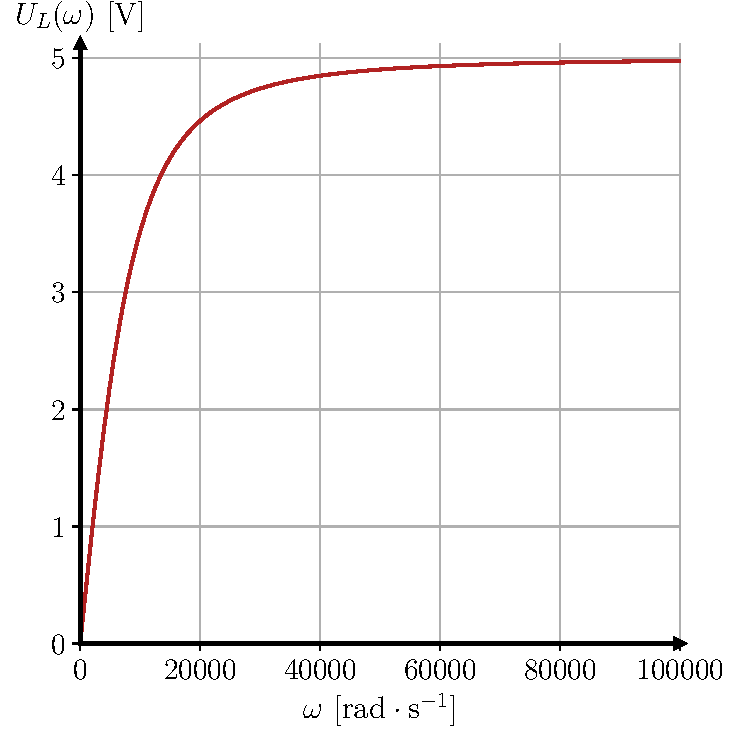
\includegraphics[width=\linewidth]{rl_Ul_ampl_prof}
		\end{center}
		\tcblower
		\begin{center}
			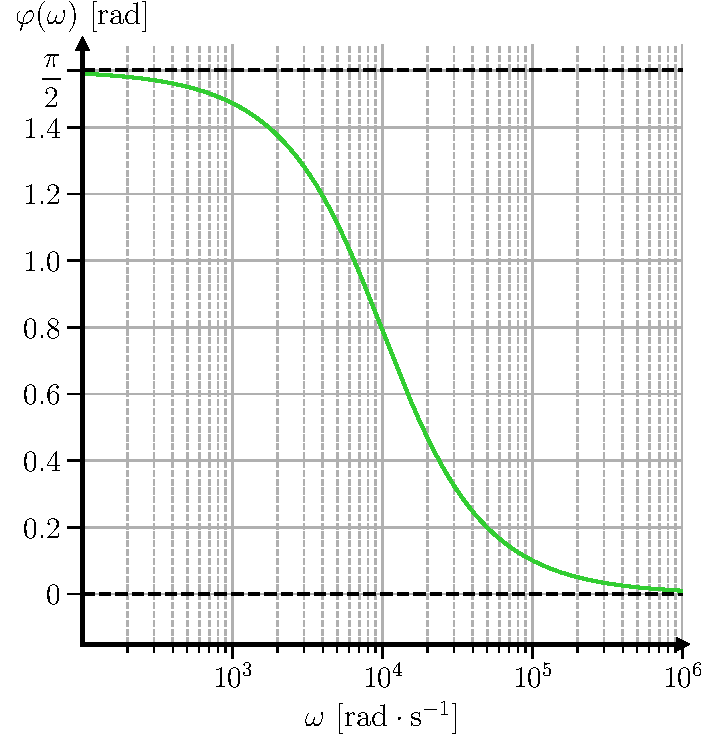
\includegraphics[width=\linewidth]{rl_Ul_arg_prof}
		\end{center}
	\end{isd}
}
\end{document}
